\chapter{Graphen}

F"ur Pfadfindung braucht man eine Traversieren zu machen. Dazu sind Graphen nutzlich (besser)...
Diese sind gut f"ur Pfadplanung bzw. Pfadfindung weil ...

\section{Navigationsnetze (\textit{eng.} Navigation Meshes)}
%\cite{Mesh:11}
%A common strategy for efficiently computing realistic
%paths is to partition the environment into a collection of
%walkable areas. This partition is often referred to as a
%navigation mesh. A useful data structure that can be used to
%construct a navigation mesh is the medial axis. The medial
%axis is the set of all points in an environment that have
%more than one distinct closest point on the boundary of the
%environment
%Proper Work
TODO

\begin{figure} %Von Website
	\centering
	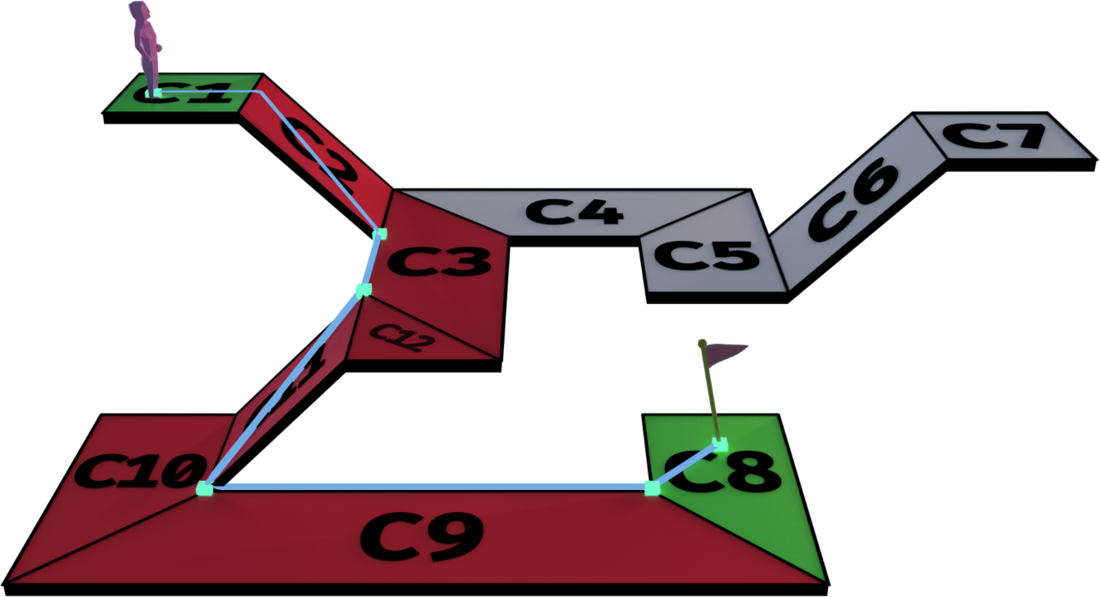
\includegraphics[width=\textwidth]{images/mesh_with_path.png}
	\caption{Von \cite{Mesh:18}: Navigation Mesh mit ein Pfad von Startpunkt C1 bis Endpunkt C2}
	\label{sec1a}
\end{figure}



\section{Rastergraph (\textit{eng.} Grid Graph)}
%A Star is good for them
%Grids are composed of tiles which lie adjacent to each other
%A raster is put on top of the environment where it will be used. Then a Graph Search with its Tiles is used to find a path in it. For that each Tile possess a travel cost. A common Pathfinding Algorthim used here is A*.
%A common Tile has 4 adjacent Tiles, however more options for a grid are possible. A hextile has six neighbours and the Octile has eight, 4 adjacent like the regular tile and 4 from diagonal movement.
%(1)
Raster bestehen aus Kacheln, die nebeneinander liegen. Laut \cite{Grid:02} wird ein Raster wird "uber die Umgebung gelegt, in der es verwendet werden soll. Dann wird eine Graphensuche mit seinen Kacheln verwendet, um einen Pfad darin zu finden. Daf"ur besitzt jede Kachel seine eigene Kosten. Die Kacheln sind Knoten und jede hat Kanten zu ihre Nachbarn. Ein "ublicher Pfadfindungsalgorithmus daf"ur ist A*.
\\\\
F"ur den Graph hat eine Kachel typischerweise 4 benachbarte Kacheln, es sind jedoch mehr Optionen m"oglich. Eine sechseckige Kachel hat sechs Nachbarn und die normale rechteckige Kachel kann 8 haben, wenn die diagonale betrachtet werden (siehe Abb. \ref{sec2a}).
\begin{figure} %Gemacht mit Paint
	\centering
	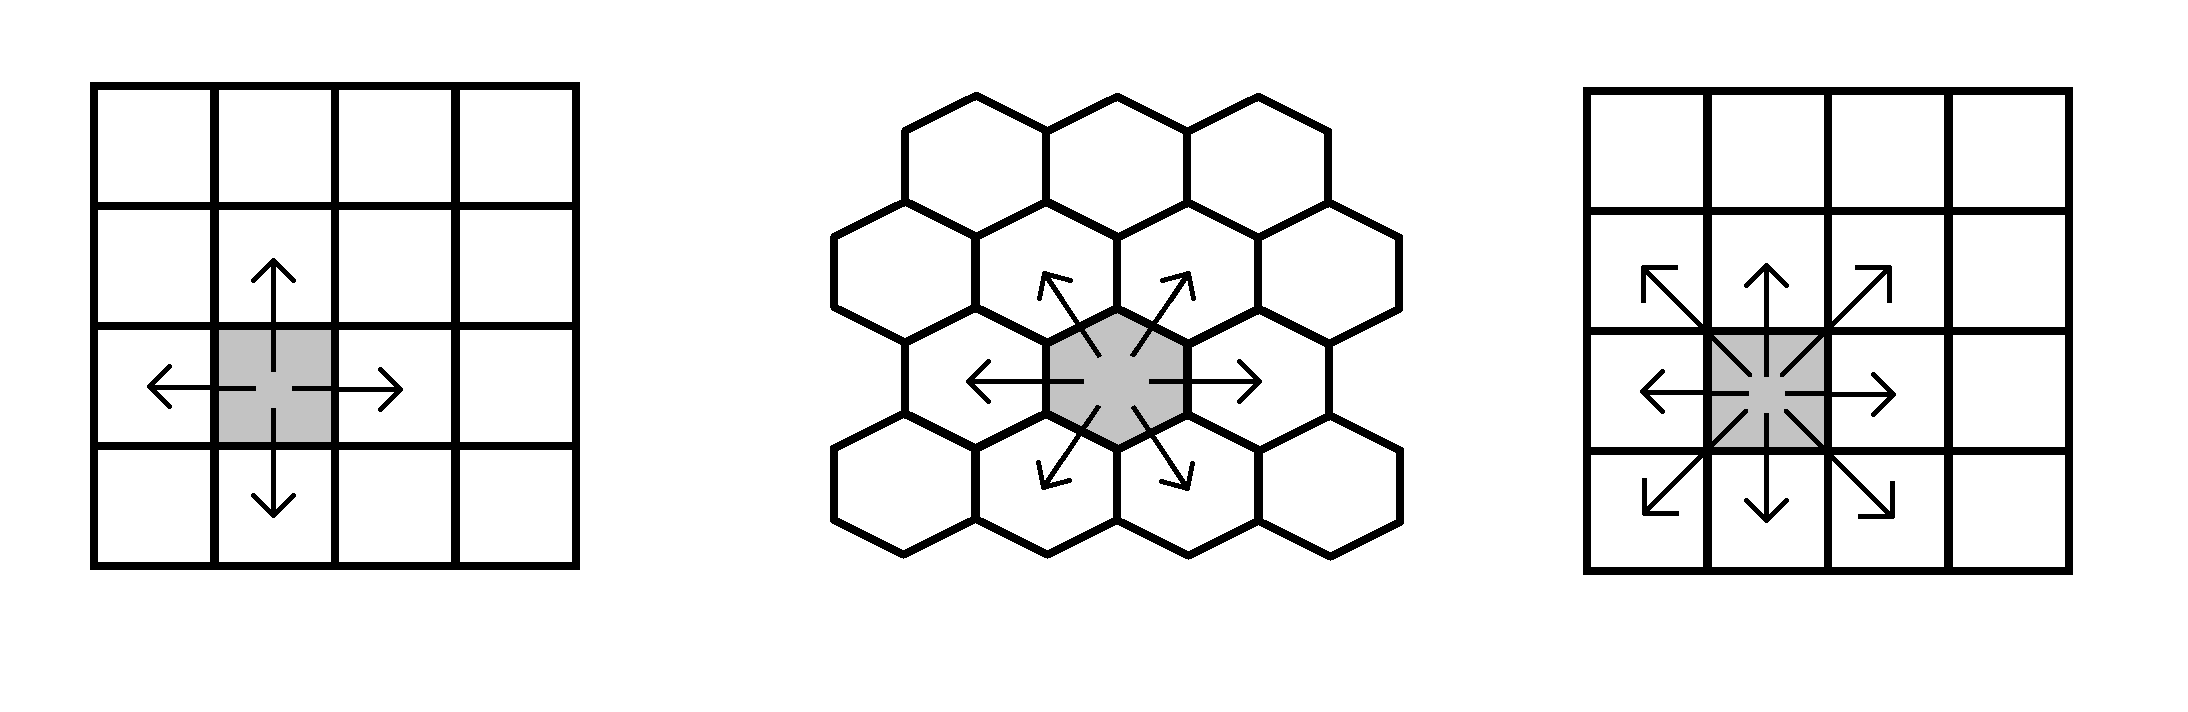
\includegraphics[width=\textwidth]{images/Grid_Tiles.png}
	\caption{Von links nach rechts: Kachel mit 4 Bewegungsoptionen, Hexagon mit 6 Bewegungsoptionen, Kachel mit 8 Bewegungsoptionen}
	\label{sec2a}
\end{figure}


\section{Sichtbarkeitsgraph (\textit{eng.} Visibility Graph)}
%(110)
%The defining characteristics of a visibility map are that its nodes share an edge if they
%are within line of sight of each other, and that all points in the robot’s free space are
%within line of sight of at least one node on the visibility map.
%
%The standard visibility graph is defined in a two-dimensional polygonal configuration
%space (figure 5.3). The nodes vi of the visibility graph include the start location,
%the goal location, and all the vertices of the configuration space obstacles. The graph
%edges ei j are straight-line segments that connect two line-of-sight nodes vi and vj , i.e.,
%Proper Work
%(110)
%Visibility graphs consist of nodes that share an edge if they are withhin line if sight with each other and no obstacle lies between them. The standard Graph is two dimensional. Possesing the start point, end point and the vertices of the polygons that represent obstacles as nodes.
%
%An example of a visibility graph lies in image ref.
%(110)
In \cite{Principles:05} ist beschrieben, dass Sichtbarkeitsgraphen aus Knoten bestehen, die sich eine Kante teilen, wenn sie in Sichtlinie zueinander stehen und kein Hindernisse zwischen ihnen liegt. Der Standardgraph ist zweidimensional. Der Startpunkt, der Endpunkt und die Eckpunkte der Polygone, die Hindernisse darstellen, werden als Knoten dargestellt.
\\\\
Ein Beispiel f"ur ein Sichtbarkeitsgraph finden Sie in Bild \ref{sec3a}.
\begin{figure} %Genommen aus Buch
	\centering
	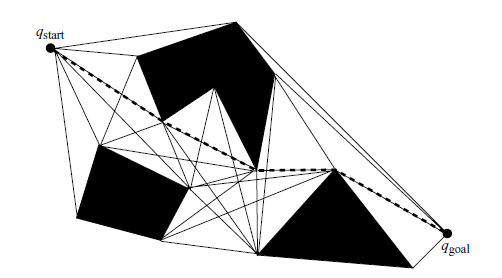
\includegraphics[width=\textwidth]{images/Robot_Motion_Visibility_Graph.png}
	\caption{Von \cite[~S. 111]{Principles:05} die Figur 5.4: Die Linien begrenzen die Kanten des Sichtbarkeitsgraph f"ur die drei als gef"ullte Polygone dargestellten Hindernisse. Die gepunktete Linie stellt den k"urzesten Weg zwischen Start und Ziel dar.}
	\label{sec3a}
\end{figure}


\section{Punktgraphen (Point Graphs)}


\section{(Automatic Navmesh Calculation)}


\subsection{Zerteilung des Navmesh (Navmesh Cutting)} 